%-------------------------------------------------------------------------------
\section{Evaluation}
%-------------------------------------------------------------------------------


\subsection{Experimental Setup}
\label{sec:expsetup}

\PN{Model and System Configuration.} 
The experiments are conducted on a system equipped with 4 NVIDIA A10 GPUs. 
The models used in this study include OPT-6.7B, OPT-13B, Qwen2-beta-7B, and Llama2-13B. 
These models were selected to represent a range of sizes and complexities, ensuring a thorough evaluation of the \sys mechanism on varying model scales. 
Unless otherwise specified, 
all experiments are conducted using a separation of the prefill and decoding phases, with each model deployed as two distinct instances: a prefill instance and a decoding instance.

\PN{Workload.} 
The workload used in the experiments is generated using a randomly designed dataloader, which allows users to customize batch size, sequence length, 
and vocabulary size based on the model requirements. Our setup can equally support real-world workloads, 
such as ShareGPT\cite{sharegpt} and Alpaca\cite{alpaca1, alpaca2} datasets, as the fundamental workload characteristics are consistent and do not significantly impact experimental results.

\PN{Baseline.} 
We consider three baselines in our evaluation: DeepSpeed, FlexGen, and a naive method.
The naive method, built upon the vLLM framework, involves loading the entire model into GPU memory without any offloading. 
Our \sys mechanism is also implemented on top of the vLLM framework, whose paged attention mechanism enables fine-grained memory management during inference.

\PN{Key Metrics.} 
We use several key metrics to evaluate performance, 
including GPU memory savings for memory efficiency, TTFT and TPOT for latency, and throughput for overall inference performance across prefill and decoding phases.


\subsection{Maintaining SLO}

We conduct experiments using the OPT-6.7B model and the Qwen2-beta-7B model with clear separation of the prefill and decoding phases to show the capability of \sys in maintaining SLO. 
The prefill phase corresponds to the TTFT SLO, while the decoding phase corresponds to the TPOT SLO. 
This separation enables us to apply different \interval values to the two instances, allowing each phase to meet its respective SLO effectively.

Due to the benefits of separation, which allows for an increased batch size in the decoding instance as we discussed earlier, we fix the batch size at 128 for the decoding instance and 32 for the prefill instance to simulate a realistic high-throughput inference scenario. 
As a baseline, we measure the performance under a naive execution mode without offloading, where the TTFT and TPOT latencies are recorded as reference points. 
Subsequently, we configured \sys to operate under varying SLO constraints for both TTFT and TPOT to test its ability to meet these requirements by adjusting the \interval parameter. 
Furthermore, we conducted experiments to compare the performance of \sys with DeepSpeed.

To ensure consistency, the SLO values are normalized to 1, 
and the recorded values represent the ratio of the observed time to the specified SLO. 
The results shown in Figure~\ref{fig:eval1} demonstrate that 
\sys effectively maintains the specified SLOs for both TTFT and TPOT in different setups. 
It further illustrates how \sys adapts to varying SLO constraints by dynamically adjusting the \interval parameter. 
When the SLO is set within the range 20\%-40\%,
the optimal \interval remains unchanged, resulting in relatively stable TPOT values. 
As the SLO increases from 40\% to 50\%, 
the optimal \interval selected during the experiment changes, 
causing a noticeable variation in the TPOT curve.

DeepSpeed suffers from significant transmission latency during inference. 
This bottleneck is particularly severe in the decoding phase, where the large volume of parameter transfers drastically amplifies the delay, 
resulting in exceeding the specified SLOs by 8.08\X and reducing its throughput by 6.8\X to 8.23\X compared to \sys.

\begin{figure}[t]
    \centering
    \resizebox{\columnwidth}{!}{
        % This file was created with tikzplotlib v0.10.1.
\begin{tikzpicture}

  \definecolor{darkgray176}{RGB}{176,176,176}
  \definecolor{green}{RGB}{0,128,0}
  \definecolor{lightgray204}{RGB}{204,204,204}
  \definecolor{orange}{RGB}{255,165,0}
  
  \begin{groupplot}[group style={group size=2 by 2, horizontal sep=2.2cm, vertical sep=2.2cm},
    title style={font=\Large},
    label style={font=\large},
    tick label style={font=\large},
    legend style={font=\large}]
    \nextgroupplot[
      legend cell align={left},
      legend style={fill opacity=0.8, draw opacity=1, text opacity=1, draw=lightgray204},
      tick align=outside,
      tick pos=left,
      title={(a) OPT Model TTFT Comparison},
      x grid style={darkgray176},
      xlabel={SLO},
      xmajorgrids,
      xmin=-0.15, xmax=3.15,
      xtick style={color=black},
      xtick={0,1,2,3},
      xtick={0,1,2,3},
      xtick={0,1,2,3},
      xticklabels={20\%,30\%,40\%,50\%},
      xticklabels={20\%,30\%,40\%,50\%},
      xticklabels={20\%,30\%,40\%,50\%},
      y grid style={darkgray176},
      ylabel={Ratio of Latency to SLO.},
      ymajorgrids,
      ymin=0.8971575, ymax=1.8429925,
      ytick style={color=black}
      ]
      \addplot [thick, orange, mark=square*, mark size=3, mark options={solid}]
      table {%
      0 0.94015
      1 0.9417
      2 0.95
      3 0.957
      };
      \addlegendentry{\sys}
      \addplot [very thick, green, dotted, mark=triangle*, mark size=3, mark options={solid}]
      table {%
      0 1.8
      1 1.67
      2 1.55
      3 1.44
      };
      \addlegendentry{DeepSpeed}
      
      \nextgroupplot[
      legend cell align={left},
      legend style={fill opacity=0.8, draw opacity=1, text opacity=1, draw=lightgray204},
      tick align=outside,
      tick pos=left,
      title={(b) OPT Model TPOT Comparison},
      x grid style={darkgray176},
      xlabel={SLO},
      xmajorgrids,
      xmin=-0.15, xmax=3.15,
      xtick style={color=black},
      xtick={0,1,2,3},
      xtick={0,1,2,3},
      xtick={0,1,2,3},
      xticklabels={20\%,30\%,40\%,50\%},
      xticklabels={20\%,30\%,40\%,50\%},
      xticklabels={20\%,30\%,40\%,50\%},
      y grid style={darkgray176},
      ylabel={Ratio of Latency to SLO.},
      ymajorgrids,
      ymin=0.48325, ymax=8.44175,
      ytick style={color=black}
      ]
      \addplot [thick, orange, mark=square*, mark size=3, mark options={solid}]
      table {%
      0 0.986
      1 0.91
      2 0.845
      3 0.9888
      };
      \addlegendentry{\sys}
      \addplot [very thick, green, dotted, mark=triangle*, mark size=3, mark options={solid}]
      table {%
      0 8.08
      1 7.46
      2 6.92
      3 6.46
      };
      \addlegendentry{DeepSpeed}
      
      \nextgroupplot[
      legend cell align={left},
      legend style={fill opacity=0.8, draw opacity=1, text opacity=1, draw=lightgray204},
      tick align=outside,
      tick pos=left,
      title={(c) Qwen Model TTFT Comparison},
      x grid style={darkgray176},
      xlabel={SLO},
      xmajorgrids,
      xmin=-0.15, xmax=3.15,
      xtick style={color=black},
      xtick={0,1,2,3},
      xtick={0,1,2,3},
      xtick={0,1,2,3},
      xticklabels={20\%,30\%,40\%,50\%},
      xticklabels={20\%,30\%,40\%,50\%},
      xticklabels={20\%,30\%,40\%,50\%},
      y grid style={darkgray176},
      ylabel={Ratio of Latency to SLO.},
      ymajorgrids,
      ymin=0.88105, ymax=2.33195,
      ytick style={color=black}
      ]
      \addplot [thick, orange, mark=square*, mark size=3, mark options={solid}]
      table {%
      0 0.947
      1 0.954
      2 0.955
      3 0.987
      };
      \addlegendentry{\sys}
      \addplot [very thick, green, dotted, mark=triangle*, mark size=3, mark options={solid}]
      table {%
      0 2.266
      1 2.09
      2 1.94
      3 1.81
      };
      \addlegendentry{DeepSpeed}
      
      \nextgroupplot[
      legend cell align={left},
      legend style={fill opacity=0.8, draw opacity=1, text opacity=1, draw=lightgray204},
      tick align=outside,
      tick pos=left,
      title={(d) Qwen Model TPOT Comparison},
      x grid style={darkgray176},
      xlabel={SLO},
      xmajorgrids,
      xmin=-0.15, xmax=3.15,
      xtick style={color=black},
      xtick={0,1,2,3},
      xtick={0,1,2,3},
      xtick={0,1,2,3},
      xticklabels={20\%,30\%,40\%,50\%},
      xticklabels={20\%,30\%,40\%,50\%},
      xticklabels={20\%,30\%,40\%,50\%},
      y grid style={darkgray176},
      ylabel={Ratio of Latency to SLO.},
      ymajorgrids,
      ymin=0.5364, ymax=8.2716,
      ytick style={color=black}
      ]
      \addplot [thick, orange, mark=square*, mark size=3, mark options={solid}]
      table {%
      0 0.962
      1 0.888
      2 0.99
      3 0.933
      };
      \addlegendentry{\sys}
      \addplot [very thick, green, dotted, mark=triangle*, mark size=3, mark options={solid}]
      table {%
      0 7.92
      1 7.32
      2 6.78
      3 6.3
      };
      \addlegendentry{DeepSpeed}
      \end{groupplot}
      
      \end{tikzpicture}
       % 插入 TikZ 图
 }
    \caption{Comparison of TTFT and TPOT between \sys and DeepSpeed under the OPT-6.7B and Qwen2-beta-7B models. 
 The y-axis represents the ratio of the observed latency to the corresponding SLO target latency, where a value of 1 indicates that the latency matches the SLO target.}
    \label{fig:eval1}
\end{figure}


\subsection{Memory Saving}
\label{sec:memsave}

We conduct experiments to evaluate and compare \sys and FlexGen in terms of memory savings and throughput performance. 
The experiments use the OPT-13B model across varying batch sizes {4, 8, 16, 32}. 
For different input scales, \sys dynamically adjusts the \interval value, while FlexGen relies on its cost model to compute the offload ratio in an attempt to minimize total latency. 
The comparison focuses on the ability of the two systems to optimize GPU memory usage and maintain high throughput under various input conditions.

Figure~\ref{fig:eval2} presents the results of the comparison. 
FlexGen's memory-saving capability is consistently inferior to that of \sys at the same batch size due to inaccuracies in its estimation of transfer and computation latencies, 
resulting in suboptimal offloading decisions. In contrast, \sys employs its analyzer to directly measure computation and data transfer times, allowing it to select the most suitable \interval and achieve 2.37\X better memory savings compared to FlexGen, thereby maximizing memory efficiency across different input scales.

Furthermore, \sys consistently achieves higher throughput than FlexGen while simultaneously delivering significantly greater memory savings. 
In the best case, \sys achieves up to 1.85\X the throughput of FlexGen. By saving more memory, \sys can support larger input scales, which further enhances throughput. 
This advantage will be discussed in greater detail in Section~\S\ref{sec:benefits}.

\begin{figure}[t]
    \centering
    \resizebox{\columnwidth}{!}{
        % This file was created with tikzplotlib v0.10.1.
\begin{tikzpicture}

    \definecolor{darkgray176}{RGB}{176,176,176}
    \definecolor{darkorange25512714}{RGB}{255,127,14}
    \definecolor{steelblue31119180}{RGB}{31,119,180}
    
    \begin{groupplot}[group style={group size=2 by 1, horizontal sep=3cm},
      title style={font=\Large},
    label style={font=\large},
    tick label style={font=\large},
    legend style={font=\large}]
    \nextgroupplot[
      legend cell align={left},
      legend style={
        fill opacity=0.8,
        draw opacity=1,
        text opacity=1,
        at={(0.03,0.97)},
        anchor=north west,
        draw=none
      },
      tick align=outside,
      tick pos=left,
      title={(a) Memory Usage on Offloading Devices},
      x grid style={darkgray176},
      xlabel={Batch Size},
      xmin=-0.535, xmax=3.535,
      xtick style={color=black},
      xtick={0,1,2,3},
      xticklabels={4,8,16,32},
      y grid style={darkgray176},
      ylabel={Memory Usage (GB)},
      ymin=0, ymax=12.5685,
      ytick style={color=black}
      ]
      \draw[draw=none,fill=steelblue31119180] (axis cs:-0.35,0) rectangle (axis cs:0,7.77);
      \addlegendimage{ybar,ybar legend,draw=none,fill=steelblue31119180}
      \addlegendentry{\sys}
      
      \draw[draw=none,fill=steelblue31119180] (axis cs:0.65,0) rectangle (axis cs:1,7.77);
      \draw[draw=none,fill=steelblue31119180] (axis cs:1.65,0) rectangle (axis cs:2,11.97);
      \draw[draw=none,fill=steelblue31119180] (axis cs:2.65,0) rectangle (axis cs:3,11.97);
      \draw[draw=none,fill=darkorange25512714] (axis cs:2.77555756156289e-17,0) rectangle (axis cs:0.35,4.672);
      \addlegendimage{ybar,ybar legend,draw=none,fill=darkorange25512714}
      \addlegendentry{FlexGen}
      
      \draw[draw=none,fill=darkorange25512714] (axis cs:1,0) rectangle (axis cs:1.35,4.8);
      \draw[draw=none,fill=darkorange25512714] (axis cs:2,0) rectangle (axis cs:2.35,5.05);
      \draw[draw=none,fill=darkorange25512714] (axis cs:3,0) rectangle (axis cs:3.35,5.57);
      \draw (axis cs:-0.2,7.97) node[
        scale=0.5,
        anchor=base,
        text=black,
        rotate=0.0
      ]{7.77};
      \draw (axis cs:0.8,7.97) node[
        scale=0.5,
        anchor=base,
        text=black,
        rotate=0.0
      ]{7.77};
      \draw (axis cs:1.8,12.17) node[
        scale=0.5,
        anchor=base,
        text=black,
        rotate=0.0
      ]{11.97};
      \draw (axis cs:2.8,12.17) node[
        scale=0.5,
        anchor=base,
        text=black,
        rotate=0.0
      ]{11.97};
      \draw (axis cs:0.2,4.872) node[
        scale=0.5,
        anchor=base,
        text=black,
        rotate=0.0
      ]{4.67};
      \draw (axis cs:1.2,5) node[
        scale=0.5,
        anchor=base,
        text=black,
        rotate=0.0
      ]{4.80};
      \draw (axis cs:2.2,5.25) node[
        scale=0.5,
        anchor=base,
        text=black,
        rotate=0.0
      ]{5.05};
      \draw (axis cs:3.2,5.77) node[
        scale=0.5,
        anchor=base,
        text=black,
        rotate=0.0
      ]{5.57};
      
      \nextgroupplot[
      legend cell align={left},
      legend style={
        fill opacity=0.8,
        draw opacity=1,
        text opacity=1,
        at={(0.03,0.97)},
        anchor=north west,
        draw=none
      },
      tick align=outside,
      tick pos=left,
      title={(b) Throughput Comparison},
      x grid style={darkgray176},
      xlabel={Batch Size},
      xmin=-0.535, xmax=3.535,
      xtick style={color=black},
      xtick={0,1,2,3},
      xticklabels={4,8,16,32},
      y grid style={darkgray176},
      ylabel={Throughput (tokens/s)},
      ymin=0, ymax=59.997,
      ytick style={color=black}
      ]
      \draw[draw=none,fill=steelblue31119180] (axis cs:-0.35,0) rectangle (axis cs:0,10.25);
      \draw[draw=none,fill=steelblue31119180] (axis cs:0.65,0) rectangle (axis cs:1,21.97);
      \draw[draw=none,fill=steelblue31119180] (axis cs:1.65,0) rectangle (axis cs:2,28.57);
      \draw[draw=none,fill=steelblue31119180] (axis cs:2.65,0) rectangle (axis cs:3,57.14);
      \draw[draw=none,fill=darkorange25512714] (axis cs:2.77555756156289e-17,0) rectangle (axis cs:0.35,8.94);
      \draw[draw=none,fill=darkorange25512714] (axis cs:1,0) rectangle (axis cs:1.35,11.85);
      \draw[draw=none,fill=darkorange25512714] (axis cs:2,0) rectangle (axis cs:2.35,25.5);
      \draw[draw=none,fill=darkorange25512714] (axis cs:3,0) rectangle (axis cs:3.35,35.46);
      \draw (axis cs:-0.2,12.25) node[
        scale=0.5,
        anchor=base,
        text=black,
        rotate=0.0
      ]{10.25};
      \draw (axis cs:0.8,23.97) node[
        scale=0.5,
        anchor=base,
        text=black,
        rotate=0.0
      ]{21.97};
      \draw (axis cs:1.8,30.57) node[
        scale=0.5,
        anchor=base,
        text=black,
        rotate=0.0
      ]{28.57};
      \draw (axis cs:2.8,59.14) node[
        scale=0.5,
        anchor=base,
        text=black,
        rotate=0.0
      ]{57.14};
      \draw (axis cs:0.2,10.94) node[
        scale=0.5,
        anchor=base,
        text=black,
        rotate=0.0
      ]{8.94};
      \draw (axis cs:1.2,13.85) node[
        scale=0.5,
        anchor=base,
        text=black,
        rotate=0.0
      ]{11.85};
      \draw (axis cs:2.2,27.5) node[
        scale=0.5,
        anchor=base,
        text=black,
        rotate=0.0
      ]{25.50};
      \draw (axis cs:3.2,37.46) node[
        scale=0.5,
        anchor=base,
        text=black,
        rotate=0.0
      ]{35.46};
      \end{groupplot}
      
      \end{tikzpicture}
       % 插入 TikZ 图
 }
    \caption{(a) Memory usage on the offloading devices for \sys and FlexGen under different batch sizes. 
 (b) Throughput comparison between \sys and FlexGen under different batch sizes.}
    \label{fig:eval2}
\end{figure}


\subsection{Profiling Accuracy}

This subsection evaluates the effectiveness of the \interval analyzer within the \sys framework, 
focusing on verifying whether the \interval value identified during the record-generating phase is indeed optimal. 
To validate this process, we perform experiments using the OPT-6.7B model with a clear separation between the prefill and decoding phases. 
This separation enables the decoding instance to adopt a larger batch size, enhancing throughput in the decoding phase. 
In our experiments, the sequence length is fixed at 64, with a batch size of 16 for the prefill instance and 128 for the decoding instance. 
We set the SLO target at 50\% and use records from the analyzer to determine the optimal \interval value. 
Subsequently, we evaluated the system's performance under non-optimal \interval configurations and recorded the corresponding GPU memory usage for each setting.

The results, shown in Figure~\ref{fig:profileraccu}, highlight the trade-offs inherent in the \interval configuration and the accuracy and necessity of the analyzer in the \sys framework. 
By generating performance records, the optimal \interval values are identified as 3 for the prefill phase and 8 for the decoding phase. 
The optimal \interval values achieve an effective balance by ensuring compliance with both TTFT and TPOT SLOs while minimizing GPU memory usage. 
When \interval is smaller than the optimal value, GPU memory usage is reduced; however, this comes at the cost of SLO violations due to increased latency, 
particularly in the TPOT phase, resulting in degraded throughput. 
In contrast, larger \interval values consistently satisfy the SLO but incur significant memory overhead without measurable performance gains. 
This inefficiency is evident in Figure~\ref{fig:profileraccu}(c), where increasing \interval results in a proportionate consumption of GPU memory while failing to improve latency or throughput.

\begin{figure*}[t]
    \centering
    \resizebox{0.8\textwidth}{!}{
        % This file was created with tikzplotlib v0.10.1.
\begin{tikzpicture}

  \definecolor{crimson2143940}{RGB}{214,39,40}
  \definecolor{darkgray176}{RGB}{176,176,176}
  \definecolor{darkorange25512714}{RGB}{255,127,14}
  \definecolor{forestgreen4416044}{RGB}{44,160,44}
  \definecolor{lightgray204}{RGB}{204,204,204}
  \definecolor{steelblue31119180}{RGB}{31,119,180}
  
  \begin{groupplot}[group style={group size=3 by 1, horizontal sep=3cm},
    title style={font=\Large},
    label style={font=\large},
    tick label style={font=\large},
    legend style={font=\large}]
  \nextgroupplot[
  legend cell align={left},
  legend style={fill opacity=0.8, draw opacity=1, text opacity=1, draw=lightgray204},
  tick align=outside,
  tick pos=left,
  title={(a) TTFT Analysis},
  x grid style={darkgray176},
  xlabel={Interval Configuration},
  xmin=-0.37, xmax=3.37,
  xtick style={color=black},
  xtick={0,1,2,3},
  xticklabels={2,3,4,5},
  y grid style={darkgray176},
  ylabel={TTFT (ms)},
  ymin=0, ymax=359.541,
  ytick style={color=black}
  ]
  \draw[draw=none,fill=steelblue31119180] (axis cs:-0.2,0) rectangle (axis cs:0.2,342.42);
  \addlegendimage{ybar,ybar legend,draw=none,fill=steelblue31119180}
  \addlegendentry{TTFT}
  
  \draw[draw=none,fill=steelblue31119180] (axis cs:0.8,0) rectangle (axis cs:1.2,229.157);
  \draw[draw=none,fill=steelblue31119180] (axis cs:1.8,0) rectangle (axis cs:2.2,223.35);
  \draw[draw=none,fill=steelblue31119180] (axis cs:2.8,0) rectangle (axis cs:3.2,210.9);
  \addplot [semithick, crimson2143940, dashed]
  table {%
  -0.37 300.9
  3.37 300.9
  };
  \addlegendentry{SLO}
  
  \nextgroupplot[
  legend cell align={left},
  legend style={fill opacity=0.8, draw opacity=1, text opacity=1, draw=lightgray204},
  tick align=outside,
  tick pos=left,
  title={(b) TPOT Analysis},
  x grid style={darkgray176},
  xlabel={Interval Configuration},
  xmin=-0.37, xmax=3.37,
  xtick style={color=black},
  xtick={0,1,2,3},
  xticklabels={5,6,8,10},
  y grid style={darkgray176},
  ylabel={TPOT (ms)},
  ymin=0, ymax=130.1265,
  ytick style={color=black}
  ]
  \draw[draw=none,fill=forestgreen4416044] (axis cs:-0.2,0) rectangle (axis cs:0.2,123.93);
  \addlegendimage{ybar,ybar legend,draw=none,fill=forestgreen4416044}
  \addlegendentry{TPOT}
  
  \draw[draw=none,fill=forestgreen4416044] (axis cs:0.8,0) rectangle (axis cs:1.2,115.03);
  \draw[draw=none,fill=forestgreen4416044] (axis cs:1.8,0) rectangle (axis cs:2.2,89.388);
  \draw[draw=none,fill=forestgreen4416044] (axis cs:2.8,0) rectangle (axis cs:3.2,68.17);
  \addplot [semithick, crimson2143940, dashed]
  table {%
  -0.369999999999999 90
  3.37 90
  };
  \addlegendentry{SLO}
  
  \nextgroupplot[
  legend cell align={left},
  legend style={
    fill opacity=0.8,
    draw opacity=1,
    text opacity=1,
    at={(0.03,0.97)},
    anchor=north west,
    draw=lightgray204
  },
  tick align=outside,
  tick pos=left,
  title={(c) Memory Usage Analysis},
  x grid style={darkgray176},
  xlabel={Interval Configuration},
  xmin=-0.63, xmax=6.63,
  xtick style={color=black},
  xtick={0,1,2,3,4,5,6},
  xticklabels={2,3,4,5,6,8,10},
  y grid style={darkgray176},
  ylabel={Memory Usage (GB)},
  ymin=0, ymax=22.96875,
  ytick style={color=black}
  ]
  \draw[draw=none,fill=darkorange25512714] (axis cs:-0.3,0) rectangle (axis cs:0.3,11.5);
  \addlegendimage{ybar,ybar legend,draw=none,fill=darkorange25512714}
  \addlegendentry{Memory Usage}
  
  \draw[draw=none,fill=darkorange25512714] (axis cs:0.7,0) rectangle (axis cs:1.3,15.8);
  \draw[draw=none,fill=darkorange25512714] (axis cs:1.7,0) rectangle (axis cs:2.3,17.25);
  \draw[draw=none,fill=darkorange25512714] (axis cs:2.7,0) rectangle (axis cs:3.3,18.69);
  \draw[draw=none,fill=darkorange25512714] (axis cs:3.7,0) rectangle (axis cs:4.3,21.125);
  \draw[draw=none,fill=darkorange25512714] (axis cs:4.7,0) rectangle (axis cs:5.3,21.5);
  \draw[draw=none,fill=darkorange25512714] (axis cs:5.7,0) rectangle (axis cs:6.3,21.875);
  \end{groupplot}
  
  \end{tikzpicture}
   % 插入 TikZ 图
 }
    \caption{The TTFT, TPOT, and memory usage of \sys under different \interval configurations. 
 The red dashed lines represent the SLO. The optimal \interval is 3 in (a) and 8 in (b).}
    \label{fig:profileraccu}
\end{figure*}


\subsection{Bandwidth contention}

We conduct experiments simulating a scenario where two GPUs share PCIe bandwidth. 
In this setup, one GPU runs the OPT-13B model while the other GPU runs the LLaMA-13B model simultaneously. 
Since both models are too large to fully fit into GPU memory, offloading strategies were required to enable the models to run successfully.
That creates a high-bandwidth contention environment as both GPUs perform offloading and data transfers concurrently. 
The sequence length was set to 64, and batch sizes of 8, 16, and 32 were tested for both tasks.

To address the contention, \sys dynamically adjusts the \interval values for both tasks, ensuring that neither exceeded the predefined SLO. 
Since it is not feasible to test the computation time in a naive mode where the entire model fits into GPU memory, we could not define the SLO as a percentage of naive execution time. 
Instead, we set the SLO as a fixed TPOT threshold of 100ms. 
This value is significantly higher than typical human reading speeds and provides a stringent and practical target for evaluating performance under high-bandwidth contention. 
We also compare the performance of \sys with FlexGen on the GPU running the OPT-13B task with the same batch sizes. 
This comparison highlights \sys's ability to adaptively manage contention on the shared PCIe bandwidth, compared to FlexGen's static offloading strategy.

The results, shown in Figure~\ref{fig:evalband}, illustrate the TPOT performance of \sys and FlexGen under varying batch sizes in a bandwidth contention scenario. 
FlexGen exhibits acceptable performance at the largest batch size tested (32) but violates the SLO at smaller batch sizes (8 and 16) due to its inability to adapt to varying PCIe transfer demands. 
In contrast, \sys consistently maintains TPOT below the SLO across all batch sizes by dynamically adjusting the \interval values of the two tasks, 
effectively mitigating bandwidth contention and ensuring balanced resource utilization. 
This adaptability enables \sys to achieve 2.9\X higher throughput compared to FlexGen at smaller batch sizes on the OPT-13B task.


\begin{figure}[t]
    \centering
    \resizebox{0.6\columnwidth}{!}{
        % This file was created with tikzplotlib v0.10.1.
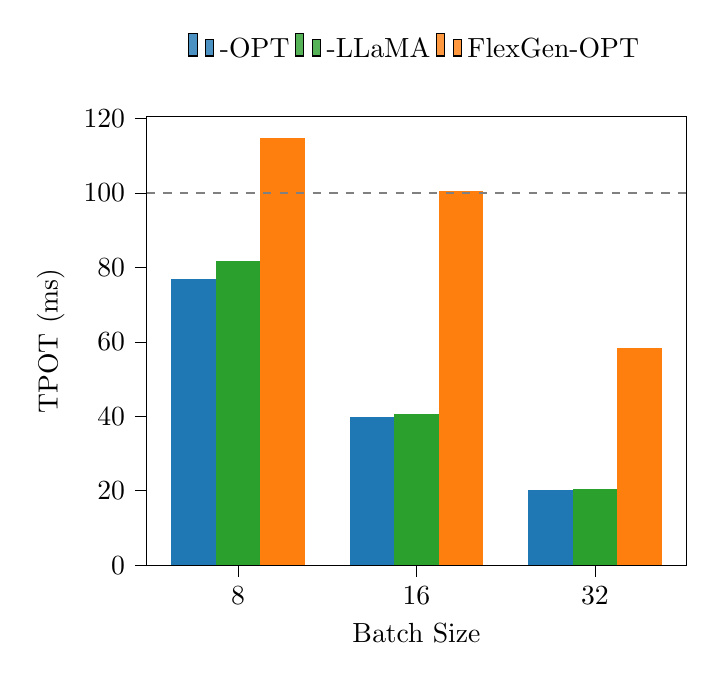
\begin{tikzpicture}

  \definecolor{darkgray176}{RGB}{176,176,176}
  \definecolor{darkorange25512714}{RGB}{255,127,14}
  \definecolor{forestgreen4416044}{RGB}{44,160,44}
  \definecolor{gray}{RGB}{128,128,128}
  \definecolor{steelblue31119180}{RGB}{31,119,180}
  
  \begin{axis}[
  legend cell align={left},
  legend columns=3,
  legend style={fill opacity=0.8, draw opacity=1, text opacity=1, at={(0.5,1.2)}, anchor=north, draw=none},
  tick align=outside,
  tick pos=left,
  x grid style={darkgray176},
  xlabel={Batch Size},
  xmin=-0.5125, xmax=2.5125,
  xtick style={color=black},
  xtick={0,1,2},
  xticklabels={8,16,32},
  y grid style={darkgray176},
  ylabel={TPOT (ms)},
  ymin=0, ymax=120.4875,
  ytick style={color=black}
  ]
  \draw[draw=none,fill=steelblue31119180] (axis cs:-0.375,0) rectangle (axis cs:-0.125,76.99);
  \addlegendimage{ybar,ybar legend,draw=none,fill=steelblue31119180}
  \addlegendentry{\sys-OPT}
  
  \draw[draw=none,fill=steelblue31119180] (axis cs:0.625,0) rectangle (axis cs:0.875,39.91);
  \draw[draw=none,fill=steelblue31119180] (axis cs:1.625,0) rectangle (axis cs:1.875,20.16);
  \draw[draw=none,fill=forestgreen4416044] (axis cs:-0.125,0) rectangle (axis cs:0.125,81.756375);
  \addlegendimage{ybar,ybar legend,draw=none,fill=forestgreen4416044}
  \addlegendentry{\sys-LLaMA}
  
  \draw[draw=none,fill=forestgreen4416044] (axis cs:0.875,0) rectangle (axis cs:1.125,40.6360625);
  \draw[draw=none,fill=forestgreen4416044] (axis cs:1.875,0) rectangle (axis cs:2.125,20.31803125);
  \draw[draw=none,fill=darkorange25512714] (axis cs:0.125,0) rectangle (axis cs:0.375,114.75);
  \addlegendimage{ybar,ybar legend,draw=none,fill=darkorange25512714}
  \addlegendentry{FlexGen-OPT}
  
  \draw[draw=none,fill=darkorange25512714] (axis cs:1.125,0) rectangle (axis cs:1.375,100.43);
  \draw[draw=none,fill=darkorange25512714] (axis cs:2.125,0) rectangle (axis cs:2.375,58.44);
  \addplot [gray, dashed, forget plot]
  table {%
  -0.5125 100
  2.5125 100
  };
  \end{axis}
  
  \end{tikzpicture}
   % 插入 TikZ 图
 }
    \caption{TPOT comparison of \sys (OPT-13B and LLaMA-13B models) and FlexGen (OPT-13B model) under contention environments across different batch sizes.
 The dashed line represents the SLO.}
    \label{fig:evalband}
\end{figure}



\subsection{Benefits of \sys}
\label{sec:benefits}

\PN{Supporting larger models.}
\sys is capable of supporting models whose memory demands exceed the GPU memory capacity, as demonstrated in experiments with the LLaMA-13B and OPT-13B models. 
Figure~\ref{fig:eval3} presents the TPOT performance of LLaMA-13B and OPT-13B, respectively, under varying batch sizes. Both models, 
which require memory beyond the 24GB GPU capacity in our setup, were successfully executed using \sys. 
TPOT values below 100 ms are higher than the normal human reading speed, indicating that such latencies allow for efficient and real-time text generation. 
In our experiments, the TPOT values for both LLaMA-13B and OPT-13B remained consistently below 100ms across all tested batch sizes, 
confirming that \sys not only enables the execution of these large-scale models but also ensures efficient performance suitable for real-world applications.

\begin{figure}[t]
    \centering
    \resizebox{\columnwidth}{!}{
        % This file was created with tikzplotlib v0.10.1.
\begin{tikzpicture}

    \definecolor{darkgray176}{RGB}{176,176,176}
    \definecolor{green}{RGB}{0,128,0}
    \definecolor{lightgray204}{RGB}{204,204,204}
    
    \begin{groupplot}[group style={group size=2 by 1, horizontal sep=3cm},
        title style={font=\Large},
    label style={font=\large},
    tick label style={font=\large},
    legend style={font=\large}]
    \nextgroupplot[
    legend cell align={left},
    legend style={fill opacity=0.8, draw opacity=1, text opacity=1, draw=lightgray204},
    tick align=outside,
    tick pos=left,
    title={OPT-13B},
    x grid style={darkgray176},
    xlabel={Batch Size},
    xmajorgrids,
    xmin=-0.25, xmax=5.25,
    xtick style={color=black},
    xtick={0,1,2,3,4,5},
    xtick={0,1,2,3,4,5},
    xticklabels={4,8,16,32,64,128},
    xticklabels={4,8,16,32,64,128},
    y grid style={darkgray176},
    ylabel={TPOT (ms)},
    ymajorgrids,
    ymin=6.4835, ymax=91.9865,
    ytick style={color=black}
    ]
    \addplot [semithick, blue, mark=*, mark size=3, mark options={solid}]
    table {%
    0 88.1
    1 44.066
    2 27.8875
    3 20.9
    4 10.46
    5 10.37
    };
    \addlegendentry{OPT-13B}
    
    \nextgroupplot[
    legend cell align={left},
    legend style={fill opacity=0.8, draw opacity=1, text opacity=1, draw=lightgray204},
    scaled y ticks=manual:{}{\pgfmathparse{#1}},
    tick align=outside,
    tick pos=left,
    title={LLaMA-13B},
    x grid style={darkgray176},
    xlabel={Batch Size},
    xmajorgrids,
    xmin=-0.25, xmax=5.25,
    xtick style={color=black},
    xtick={0,1,2,3,4,5},
    xtick={0,1,2,3,4,5},
    xticklabels={4,8,16,32,64,128},
    xticklabels={4,8,16,32,64,128},
    y grid style={darkgray176},
    ylabel={TPOT (ms)},
    ymajorgrids,
    ymin=6.4835, ymax=91.9865,
    ytick style={color=black},
    % yticklabels={}
    ]
    \addplot [semithick, green, mark=*, mark size=3, mark options={solid}]
    table {%
    0 87.5
    1 43.5
    2 27.5
    3 20.5
    4 10.8
    5 10.6
    };
    \addlegendentry{LLaMA-13B}
    \end{groupplot}
    
    \end{tikzpicture}
     % 插入 TikZ 图
 }
    \caption{TPOT of OPT-13B and LLaMA-13B models using \sys.}
    \label{fig:eval3}
\end{figure}

\PN{Supporting more input and output tokens.}
To evaluate the capability of \sys in generating longer output sequences and supporting larger batch sizes and/or sequence lengths, we leverage a critical metric:
the maximum allocatable length (\textit{max length}). 
This metric is computed as 
\[
\textit{max length} = \textit{batch size} \times (\textit{sequence length} + \textit{output length}),
\]
where the term captures the total number of tokens that the system can handle for a single model instance. 
The \textit{max length} is directly determined by the number of GPU blocks allocatable via the vLLM backend, which dynamically manages GPU memory to optimize allocation. 
A higher \textit{max length} indicates the system’s ability to support larger batch sizes, longer input sequences, and extended output sequences.

In our experiments, we use the Qwen2-beta-7B model, which supports a maximum position embedding size of 32,768 tokens. 
This choice is deliberate, as Qwen2-beta-7B significantly exceeds the position embedding limits of other models like OPT and LLaMA, 
ensuring that the system remains capable of processing long input sequences without being constrained by the model's internal architecture. 

The results in Figure~\ref{fig:eval4} show that, by adjusting the offloading intervals, \sys achieves varying degrees of memory savings for model inference. 
When the interval value is smaller, a larger proportion of the model's parameters is offloaded to CPU memory, significantly reducing the GPU memory footprint. 
This allows \sys to allocate more GPU memory for token processing, thereby increasing the maximum allocatable length. 
As a result, the system can support larger batch sizes, longer input sequences, or extended output sequences under smaller interval settings, which helps to improve throughput.


\begin{figure}[t]
    \centering
    \resizebox{0.5\columnwidth}{!}{
        % This file was created with tikzplotlib v0.10.1.
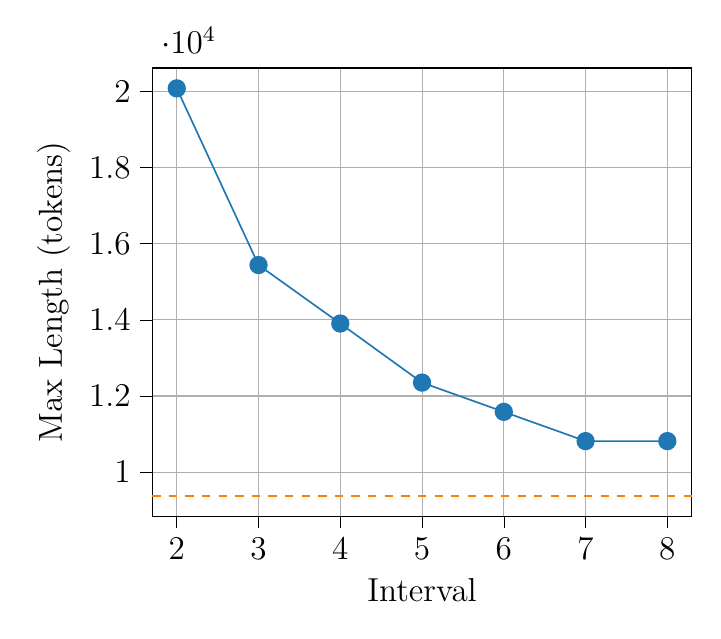
\begin{tikzpicture}

    \definecolor{darkgray176}{RGB}{176,176,176}
    \definecolor{darkorange25512714}{RGB}{255,127,14}
    \definecolor{steelblue31119180}{RGB}{31,119,180}
    
    \begin{axis}[
        title style={font=\Large},
        label style={font=\large},
        tick label style={font=\large},
        legend style={font=\large},
    tick align=outside,
    tick pos=left,
    x grid style={darkgray176},
    xlabel={Interval},
    xmajorgrids,
    xmin=1.7, xmax=8.3,
    xtick style={color=black},
    y grid style={darkgray176},
    ylabel={Max Length (tokens)},
    ymajorgrids,
    ymin=8840.8, ymax=20615.2,
    ytick style={color=black}
    ]
    \addplot [semithick, steelblue31119180, mark=*, mark size=3, mark options={solid}]
    table {%
    2 20080
    3 15440
    4 13904
    5 12352
    6 11584
    7 10816
    8 10816
    };
    \addplot [semithick, darkorange25512714, dashed]
    table {%
    1.7 9376
    8.3 9376
    };
    \end{axis}
    
    \end{tikzpicture}
     % 插入 TikZ 图
 }
    \caption{Maximum prompt length the model can process under different \interval settings.
 The dashed line represents the maximum length in the naive mode.}
    \label{fig:eval4}
\end{figure}

